\title{Planning \& Design Report}
\author{
	\textbf{Group 7} \\ \\
	Harry Stevenson \\
	Stephen Lynn \\
	David Todd \\
	Liam Joy \\
	Thomas Gak Deluen
}

\documentclass[11pt, oneside, a4paper]{article}
\usepackage[table, xcdraw]{xcolor}
\usepackage{graphicx}
\usepackage[margin=1in]{geometry}
\usepackage{mathtools}
\usepackage{multicol}
\bibliographystyle{plain}

\begin{document}

\clearpage
\maketitle
\thispagestyle{empty}

\newpage
\setcounter{page}{1}

\section{Abstract}

This document outlines the design of the system that will meet the requirements
outlined in the Requirements Analysis report for the stakeholders, Deutsche Bank.
The system will serve alert the stakeholders to irregularities and anomalies in
simulated streams of FTSE 100 stock market data. This solution will be using general
statistical analysis methods which can be applied to any field to detect anomalous
data, but will be specialised in this case for analytics of trading data. In a real
life case, the trading data will be much richer in information, however the same
analytical methods will still apply.

\section{Group Communication}

To communicate between everyone in the group, we will utilise Slack. The coding
done shall be pushed to our private repository on Github for a centralised code
base and its version control. We will use Google Drive and Google Docs for sharing
reports, so all team members can work simultaneously on the same document.

\section{Software Methodology}

We have chosen to adopt an agile methodology to development, with
a scrum approach. We decided that the ideal time to have a sprint planning session
would be at the beginning of every week, commencing after the planning and design
document has been finalised. Given the time constraints of the project, a longer
gap between sprint sessions would make an iterative approach more difficult. We
chose this methodology over the classical waterfall approach as it permits a greater
level of interaction with the customer and therefore allowing the system to better
meet the project requirements. In addition, it allows us to first perfect the basic
functionality of the system before adding additional features.

\section{Backend}
\subsection{Programming Languages}

The backend of the software shall be written in Python. We chose this as it offers
a large variety of machine learning libraries to choose from, such as
sci-kit learn. Python has a very simple and straightforward syntax, which will
increase the readability of our code. A large part of the backend of this project
is statistical analysis of data. Python balances strong statistical analysis with
general purpose usage, a purely statistical language such as R would not suffice.

The system will use a RethinkDB database. This is a NoSQL document-based database,
well suited for realtime web applications. It allows the frontend to listen for
changes, such as update, delete or insert, therefore producing quick updates to
the user when the backend receives real-time market data or sends an alert. This
is an important aspect of our system which requires traders to make quick, informed
decisions. RethinkDB also has official drivers for Python and JavaScript, which
simplifies the process of connection to the database for backend analytics.

\subsection{Backend Workflow}

As can be seen in the activity diagram in figure \ref{ActivityDiagram},
each trade is read, either from the live data feed or the static file, then placed
into the database. Then, each row is analysed using the above statistical methods.
If these methods indicate an irregularity, an alert is triggered on the front end
for the user. Otherwise, the current running averages are updated to take the new
row into account.

\begin{figure}[h]
	\centering
		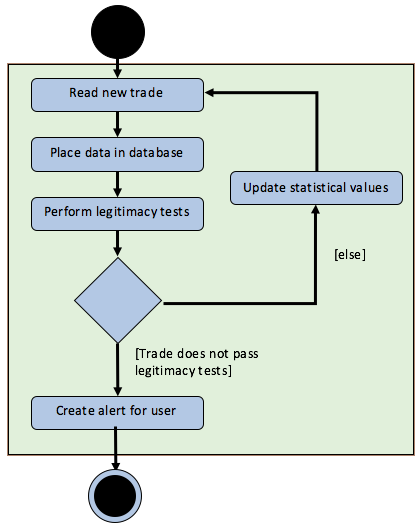
\includegraphics[width=200px]{ActivityDiagram.png}
	\caption{Activity diagram to show the flow of data coming in and out of the system}
	\label{ActivityDiagram}
\end{figure}

\subsection{Anomalous Data Detection}

We visualised the sample data that we have been given using histograms to plot
the frequency of particular values such as trade sizes or the change in price
between trades. We found this data gave a skewness between -1 and 1. Thus, the
data can be assumed to be normally distributed and can be modelled using the
normal distribution. The following formulae will be used for calculations:\\

\textit{Mean: } $\mu = \frac{\sum_{i=1}^{N} x_{i}}{N}$

\textit{Standard Deviation: } $\sigma = \sqrt{\frac{1}{N}\sum_{i=1}^{N}(x_{i} - \mu)^2}$

\textit{Expected Frequency Outside Range $=$ 1 in }$\frac{1}{1-erf(\frac{x}{\sqrt{2}})}$

\textit{Where Range }$ = \mu \pm x\sigma$

\textit{Where erf(x) } = $\frac{2}{\sqrt{\pi}}\int_0^x\mathrm{e}^{-x^2}$\\

As stated by the Empirical Rule (68-95-99.7), 99.7\% of the data should lie in the
range $\mu \pm 3\sigma$. The above formulae shows that a value that lies outside
the above range should occur only once every approximately 370 values:\\

\textit{1 in }$\frac{1}{1-erf(\frac{x}{\sqrt{2}})} \implies $ \textit{1 in }$\frac{1}{1-erf(\frac{3}{\sqrt{2}})} = $ \textit{1 in }$\frac{1}{1-0.9973...} = $ \textit{1 in }$370.37... \approx $ \textit{1 in 370} \\

This is a good basis to begin to detect anomalous data from.

Other anomalies will involve an increase/decrease in mean values for the size/price
of trades. This could indicate fraudulent practices such as pump and dumps or bear
raids. Volume spikes could also be picked up by analysing a change in size of trades
for particular company stocks. Using statistical analysis methods like the ones
described above could flag a variety of anomalies in the data.

\begin{figure}[h]
	\centering
		\includegraphics[width=200px]{StatisticalHistogram.png}
	\caption{Histogram showing the price change against frequency and the fit of the normal distribution}
	\label{StatisticalHistogram}
\end{figure}

The histogram in figure \ref{StatisticalHistogram}, constructed from the supplied
data, where the price of a trade of a single stock is compared to the previous
trade price of that stock to find the difference between trades. The data has a
skewness of 0.0113 and so can be assumed as normally distributed. This is an
example of how you can detect anomalies that occur at the very edges of the graph
as they are least likely to occur naturally.

As a stretch goal for our project, we will attempt to categorise these different
anomalies so that our program can learn from the data and alert the user to a possible
reason for the anomaly. This could include distinguishing between a volume spike and
an intended artificial inflation of a stock seen in pump and dumps, both would raise
the price of a stock and therefore may appear at first to be similar anomalies.

\subsection{Machine Learning Algorithm}

For our predictions and some of our analysis, our system will use linear regression
to find a line of best fit between our data points. The line will be of the form
$y=mx+c$ with $m$ and $c$ being calculated like so:
\begin{align*}
		& m=\frac{\bar{x}.\bar{y} - \bar{xy}}{(\bar{x})^2 - \bar{x^2}}&
		&&
		c=\bar{y} - m \bar{x}
		&&
\end{align*}

Where $\bar{x}$ is the mean of all $x$ values of our data points, and $\bar{y}$ is the
mean of all $y$ values of the data points. $X$ values will be representing time, and
$Y$ values will represent the stock characteristics such as prices and volume. Once
we have this line, we will be able to extend it beyond our current data to enable
us to predict future $Y$ values, within a range. Since we will be using unpredictable
data that can change rapidly, we will vary the size of the set of data points, thus
the predictions for future prices will be in the form of a range of values. We will
allow the user to define how many trades are used for this analysis and prediction,
in turn defining the base size of our sets.

After we have our best fit line, we’ll then be able to calculate how volatile or
stable each stock is. We’ll do this by comparing our actual values to our predicted
ones to find the average error $e$. This formula is shown below:
\begin{align*}
	&e=\frac{\sum_{i=1}^{n}|y_i - (mx_i + c)|}{n}&
\end{align*}

In our program we will compare each stock’s average error to determine its volatility.

\subsection{Class Interaction}
Our design features many elements that must work together, the UML class diagram
in figure \ref{ClassDiagram} illustrated the relationships between different
entities in the system.

The system will have many trades, each for which, two traders with unique ID's
will be associated, the buyer and seller. The trade itself will have the attributes
as taken from the data stream and have associated methods to compare the price or
size or the new trade compared to the statistical data. If the trade does not pass
the test against the statistical data, then that one trade will invoke one alert
consisting of the stock that was being traded along with the type of anomaly that
the offending trade may be categorised as, this alert may then be either approved
or rejected. For each single stock there will exist multiple trades and multiple
alerts, here each stock will have attributes such as the average price and a
trendline which will be used to perform the statistical analysis as well as making
predictions based on previous, historical data. A stock may have multiple days of
this historical data consisting of the open and close price for the relevant days.

\begin{figure}[h]
	\centering
		\includegraphics[width=300px]{UMLClassDiagram.png}
	\caption{UML class diagram to show how the different entities in the system will interact with each other}
	\label{ClassDiagram}
\end{figure}

\section{Frontend}
\subsection{Programming Languages}
We decided that a web application for the front end would offer the greatest level
of usability, providing a clear and concise interface to detail the data analysis.
In addition to this, it means that it will be compatible with a large range of
devices.

The backend and frontend are only connected through the database, leaving room for
future changes. If the stakeholders require a different frontend, altering it will
be possible without alterations to the backend. Furthermore, a web portal is easily
accessible for a large team of users, each with different roles. The specification
requires that the system must be suitable for non technical users, and a web-based
interface offers an intuitive, user friendly environment to suit such users.

We will build the front-end using JavaScript, to allow for rapid prototyping and
real-time updates to the site, alongside it being both fast to execute and fast
to write. Furthermore, JavaScript has many prewritten environments, frameworks
and applications, which allow us to quickly implement our system with widely used
applications.

\subsection{Frontend Architechture}
The frontend runs in a simple NodeJS app. This uses ExpressJS to handle the
different aspects of the server such as routing and static assets. This couples
with a ready to use real-time web framework Horizon. Horizon allows the client to
connect to the server through websockets to listen for changes in the database.

We will build the client using ReactJS, a fast and reliable user-interface framework
that uses a virtual DOM. This removes the need for DOM manipulations: when the state
changes, the required components of the client are redrawn, allowing rapid changes in
the database to be quickly propagated to the view. ReactJS is component-based which
gives the ability to write components for each part of the client, make testing more
in-depth and component specific, allowing bugs to be quickly found and changes in
the code to have fewer side-effects as each component works independently, with most
components being stateless and presentational. We will write the JavaScript in high
level ES7 code and compile it using the Babel compiler. This will maximise the number
of supported browsers. It also allows us to test our code every time we compile it.

\subsection{Customer Interaction}
Our site will consist of three main pages; the homepage, where the user can immediately
access their alerts and upload static files. The alerts page, where the system holds
every alert for review, along with previous saved alerts. The stocks page, where
the user can analyse the performance of all the FTSE 100 stocks. The page includes
statistics such as volatility and average stock price alongside short-term stock
price predictions. This is illustrated in figure \ref{UseCase}. Mockup design images
for each web page in our system are included in the appendix.

\begin{figure}[h]
	\centering
		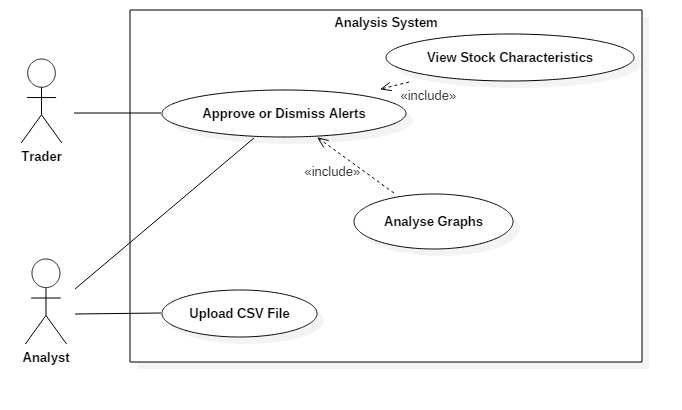
\includegraphics[width=300px]{UseCaseDiagram.png}
	\caption{UML use case diagram}
	\label{UseCase}
\end{figure}

\section{Architectural Pattern}
For this project, we will use the Pipe and Filter architectural pattern. In this
case, data is input into the backend, processed, then written to the database.
The frontend then reads the data from the database, in addition to receiving data in
the form of a CSV file from the customer, which it passes to the backend for analysis.
This is illustrated in figure \ref{ArchitechturalPattern}.

\begin{figure}[h]
	\centering
		\includegraphics[width=300px]{ArchitecturalPattern.png}
	\caption{UML architchtural pattern diagram showing how data will progress through the system}
	\label{ArchitechturalPattern}
\end{figure}

To keep maintain high uptime and prevent the front end from hanging, once a user
uploads a file to the front-end, the frontend writes it to the disk and a forks a
background task to analyse the file. Once the backend launches the task, the front-end
server lets the user know the file is currently undergoing analysis. The system
notifies the user in real time of the file’s analysis.

\section{Extensibility}
The nature of the specification lends the system to further extension. We designed
the software so that further statistical analysis can be done on the data if it is
required. The agile approach to development will help us to construct the software
in this way.

The largest problem faced by the system with regard to extensibility is the storage
space required to store all of the trade data. In a CSV file format, one day of
trade data is approximately 100MB, around 800,000 rows. This means that when the
system is run, it must be run on a machine with a large memory capacity and a high
read/write speed.

This system is intended as a model for finding anomalous data. In a real life case,
the data received from the stock market will be much richer in information, however
we can use the same fundamental principles implemented in this solution to analyse
richer data, and identify different anomalies.

\section{Robustness}
The system only has two forms of input, a static CSV file, and a live data feed.
The live data feed will always be in the same format, so we do not need to validate
it. If the CSV file inputted is not correctly formatted, the program will not analyse
it, and display a formatting error to the user. Changes to the extraction of the
data are simple, as the format used for this project has been simplified for this
task, so this can be easily extended to handle more verbose data.

The system will be robust with regard to the live feed of data. As the connection
is open, we will check the connection’s activity frequently, and upon disconnection,
it will reconnect as soon as possible, so as little data is lost as possible.

\section{Reliability}
We will measure the reliability of the system through the consistency of alerts.
The alerts will appear within 5 seconds of the analysis of the offending trade,
or final trade in a set of trades. We will multithread the backend Python so that
we can analyse many trades can at once, ensuring that the analytics will be able
to keep up with the live feed of data. Furthermore, the RethinkDB database ensures
high-speed communication between the frontend and backend. It is able to alert the
front end immediately after we detect anomalous activity. In this project, the
underlying DB acts as both storage, and a bidirectional messenger between both the
frontend and the backend.

\section{Correctness}
After we build each iteration of the software, we will analyse that iteration to
see what requirements it meets, and whether it should have met any other requirements.
This is in addition to the unit tests that we will perform at each stage throughout
development. This allows us to shape future iterations in a customer driven manner,
ensuring that we meet every requirement.

\section{Compatibility \& Portability}
The system will be compatible with a wide range of platforms, including mobile
devices, as we are using a web application. We chose this due to the requirements
stating that the system should be developed for a wide range of non-technical users.
The higher the number of users, the more practical a web application becomes, as
long installations are not necessary. The backend of the system should run on a
single server. Slow disk access can cause a bottleneck in the speed of the system.

\section{Modularity \& Reuse}
We designed both the backend and frontend in a modular way, so that they only
interact through the database. This means that both the frontend and the backend
are entirely changeable, provided they write to the database in the same format
as the current system.

\section{Security}
There are no plans in the system to implement a user access system, as this is out
of scope of the project’s requirements. This means that whoever is able to access
the web portal has access to all  the analysis of the live feed’s data. However,
this software only serves as a model to provide data analysis. The stakeholders
can implement security aspects of the software when they receive the final product.
For example, the system could only be accessible through the stakeholder’s local
network or virtual private network. Access to the system could be incorporated
into an SSO (Single Sign On) system that may already used by the stakeholders for
other means. Security considerations that arise from the creation of the software
are out of the scope of this project.

\section{Testing Plan}
We will test our Python code using built-in unit tests. Unit tests allow early
spotting of logical errors as well as checking whether the modules function as
intended.

We will also test our JavaScript code using different testing methods as React
components display as HTML. Because the JavaScript code is compiled, any syntactic
errors are quickly spotted. Therefore additional tests serve to verify the code’s
semantic behaviour. After each sprint planning session, we will run manually
created unit tests to analyse manually created data designed trigger certain
functionalities of the software.

As we are developing the frontend and backend as separate entities, the system
requires integration testing to make sure that they can both communicate data
between them.

\newpage
\begin{thebibliography}
	\item Facebook {\em React} \\
	https://facebook.github.io/react/ \\
	Date Accessed: 09/02/2017
	\item Nodejs {\em Expressjs} \\
	http://expressjs.com/ \\
	Date Accessed: 09/02/2017
	\item Nodejs {\em Docs} \\
	https://nodejs.org/en/docs/ \\
	Date Accessed: 09/02/2017
	\item RethinkDB {\em RethinkDB Horizon Docs} \\
	http://horizon.io/docs/ \\
	Date Accessed: 09/02/2017
	\item RethinkDB {\em RethinkDB} \\
	https://www.rethinkdb.com/ \\
	Date Accessed: 09/02/2017
	\item Weisstein, Eric {\em Erf} \\
 	http://mathworld.wolfram.com/Erf.html\\
	Date Accessed: 09/02/2017
	\item Niles, Robert {\em Standard Deviation} \\
	http://www.robertniles.com/stats/stdev.shtml \\
	Date Accessed: 09/02/2017
	\item Andale {\em Statistics How To} \\
	http://www.statisticshowto.com/empirical-rule-2/ \\
	Date Accessed: 09/02/2017
	\item Bas, Ryan {\em React Reconciliation} \\
	https://dev.to/ryanbas21/react-reconciliation \\
	Date Accessed: 09/02/2017
	\item Weisstein, Eric {\em Linear Regression} \\
	http://mathworld.wolfram.com/LinearRegression.html \\
	Date Accessed: 09/02/2017
\end{thebibliography}

\newpage
\appendix
\section{Gantt Chart & Activity Network}

\begin{figure}[h]
	\centering
		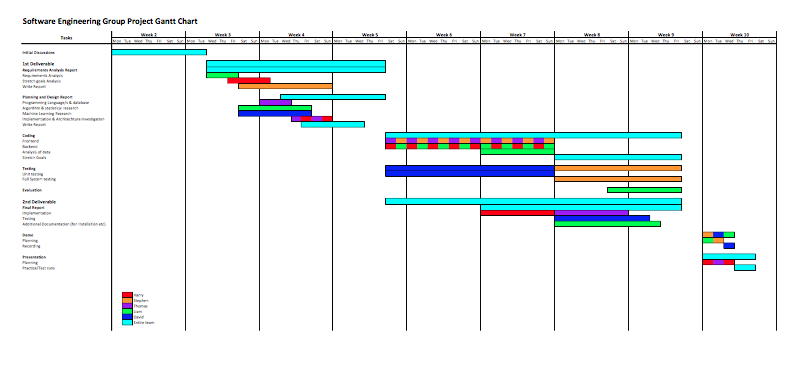
\includegraphics[width=300px]{Gantt&Activity.png}
	\caption{}
	\label{GanttActivity}
\end{figure}

\section{Risk Register}

\begin{figure}[h]
	\centering
		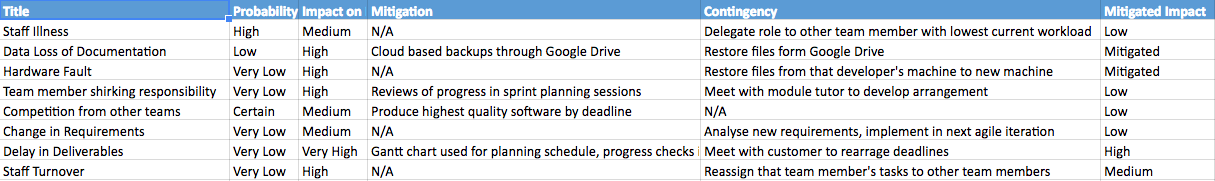
\includegraphics[width=500px]{RiskRegister.png}
	\caption{}
	\label{RiskRegister}
\end{figure}

\section{User Interface Designs}

\subsection{Homepage}

\begin{figure}[h]
	\centering
		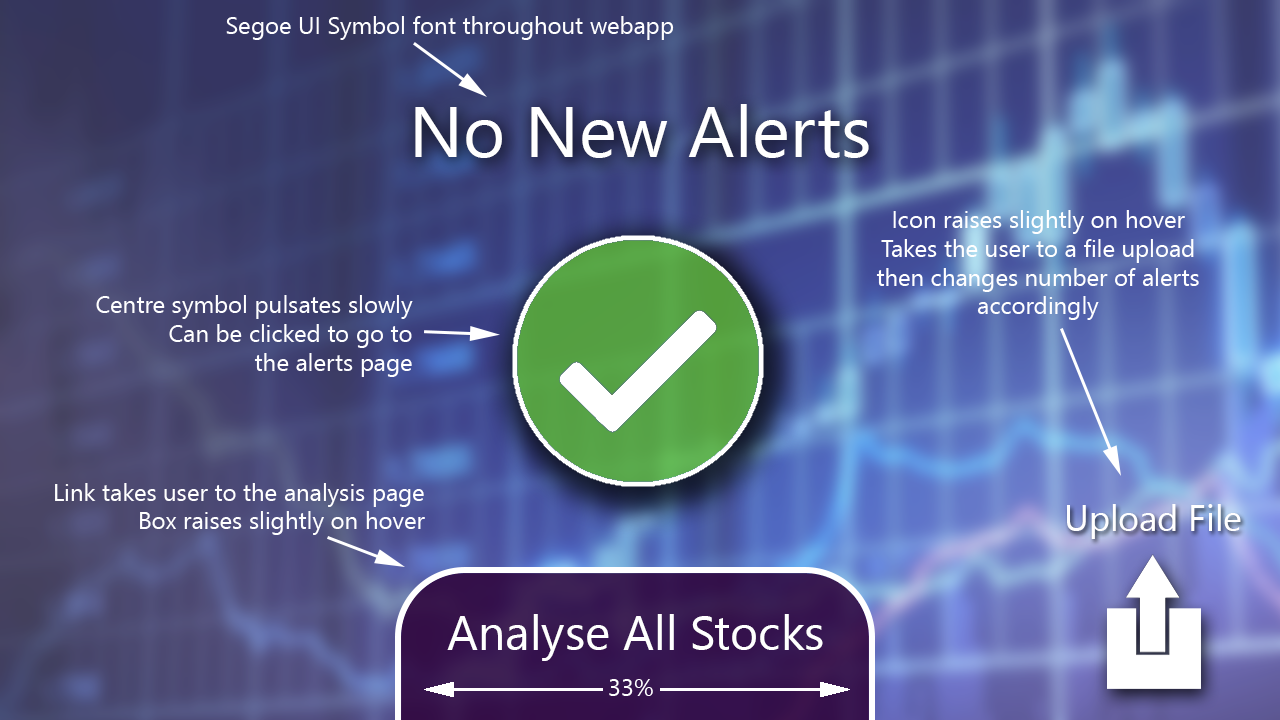
\includegraphics[width=300px]{HomepageUIDesign.png}
	\caption{}
	\label{HomeUI}
\end{figure}

\begin{figure}[h]
	\centering
		
\includegraphics[width=300px]{HomepageUIDesignAlerts.png}
	\caption{}
	\label{HomeUIAlerts}
\end{figure}

\subsection{Alerts Page}

\begin{figure}[h]
	\centering
		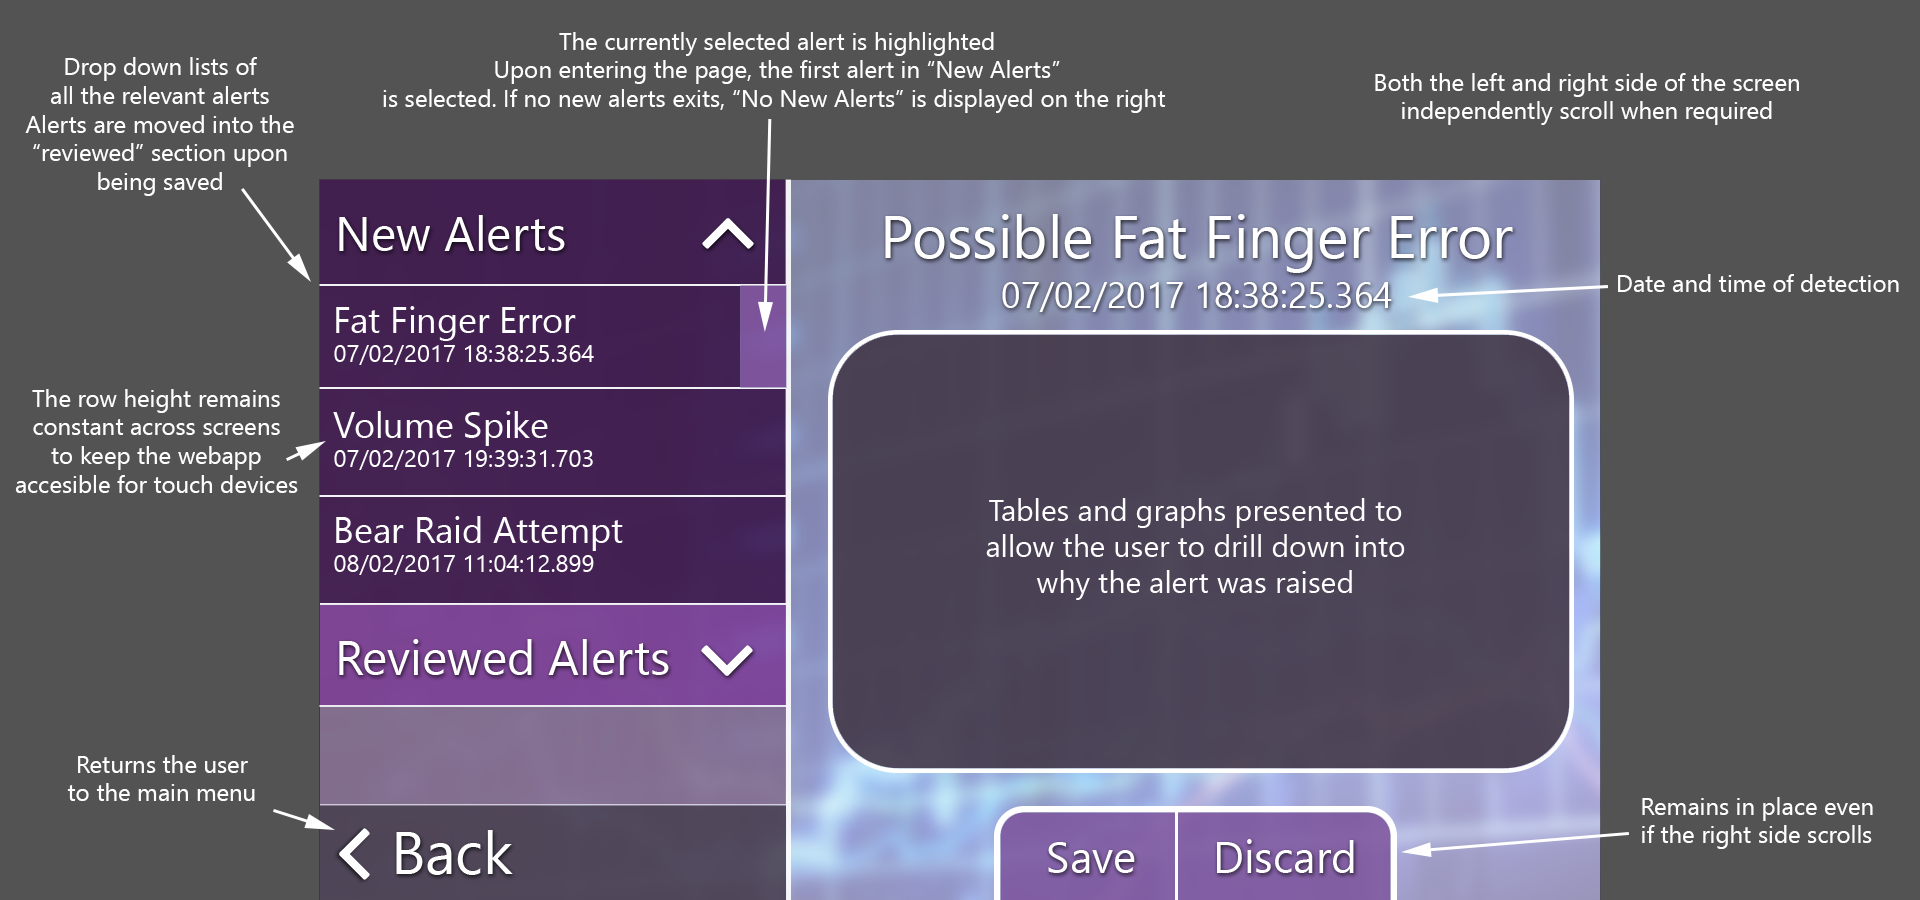
\includegraphics[width=300px]{AlertsUIDesign.png}
	\caption{}
	\label{AlertsUI}
\end{figure}

\subsection{Stocks Page}

\begin{figure}[h]
	\centering
		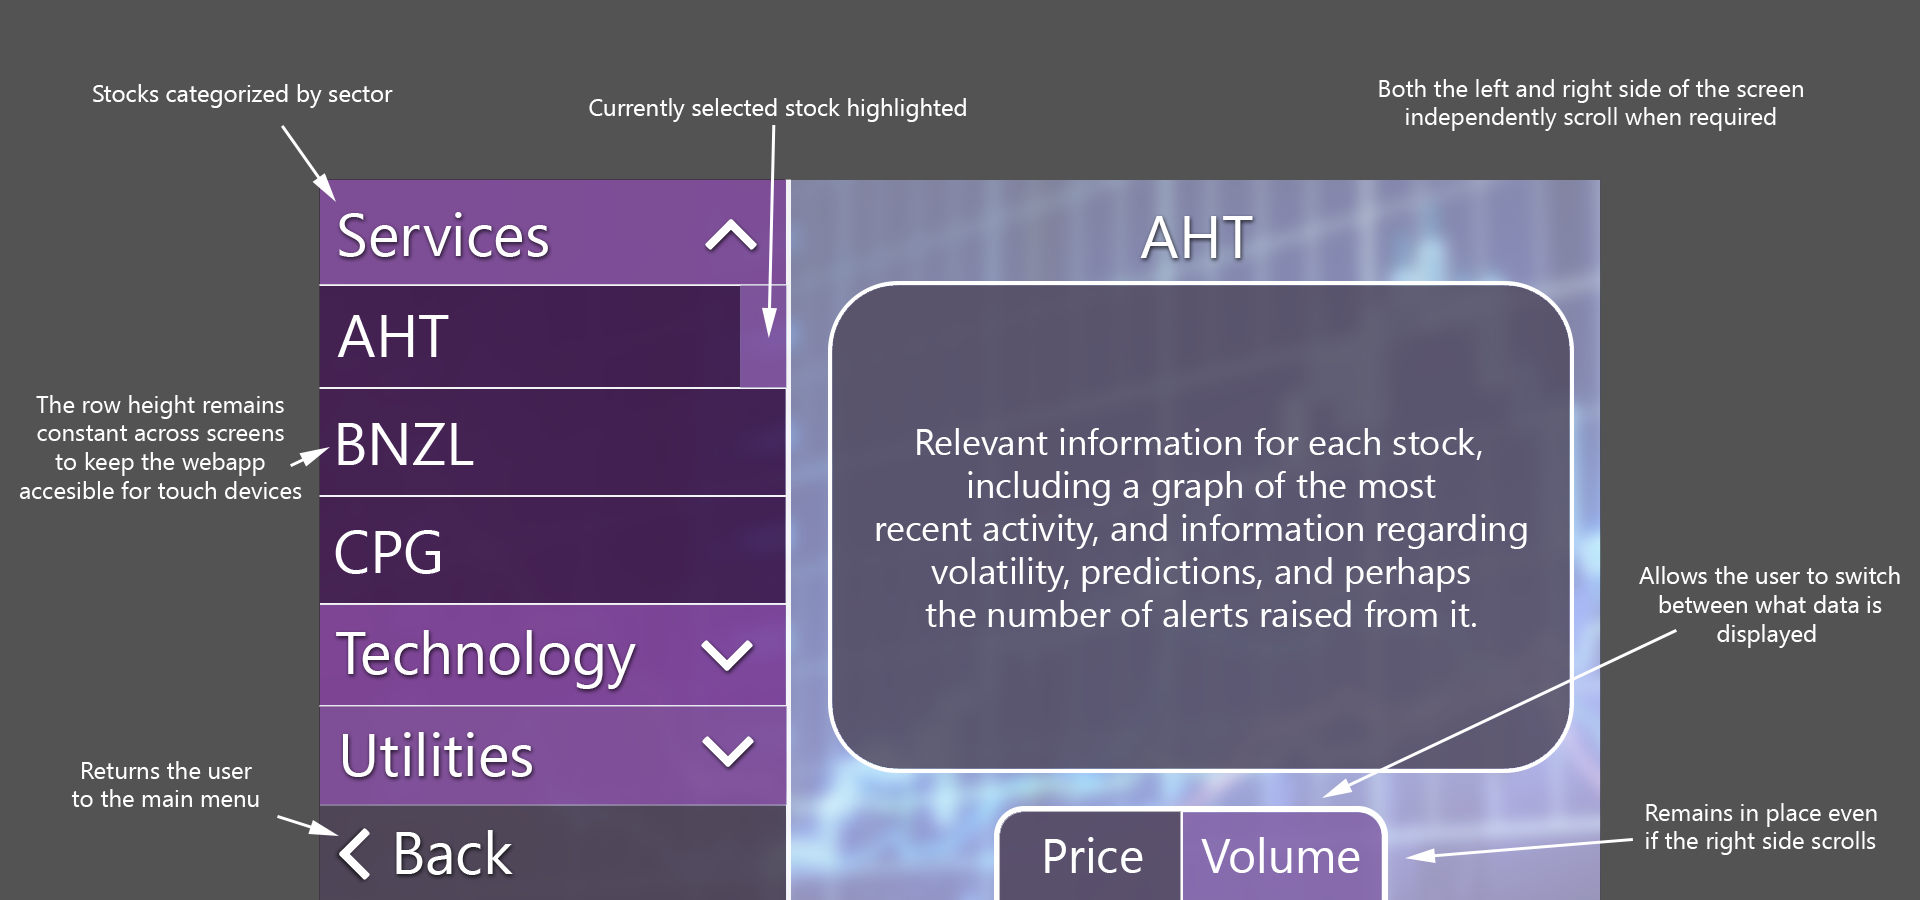
\includegraphics[width=300px]{StocksUIDesign.png}
	\caption{}
	\label{StocksUI}
\end{figure}

\end{document}
